\chapter{ANALISIS DAN PERANCANGAN}

Bab ini menjelaskan mengenai detil analisis masalah dan solusi pendekatan penyelesaiannya yang diambil di tugas akhir ini.

\section{Analisis Masalah}

Dari studi yang sudah diteliti, didapat bahwa walaupun sudah cukup banyak studi yang membahas mengenai algoritma estimasi \textit{world model} yang melacak posisi robot maupun bola di kontes robot sepak bola, hampir semua studi tersebut mengasumsikan bahwa komunikasi antar robot memiliki latensi yang dapat diabaikan. Studi yang melakukan pengujian pada kasus kegagalan komunikasi berjumlah sedikit dan juga hanya menguji kasus kegagalan komunikasi total pada suatu robot. Banyak algoritma yang dibahas dari studi sebelumnya tidak dapat bekerja secara efektif dalam keadaan latensi komunikasi yang signifikan, seperti teknik merata-ratakan data, menggabungkan distribusi Gaussian data, maupun melakukan minimasi \textit{error} terhadap sistem. Algoritma \citet{ahmad2017} dibahas sebagai algoritma yang bersifat \textit{online} yang tidak membutuhkan terkumpulnya informasi dari robot-robot lainnya sebelum suatu robot dapat mulai melakukan kalkulasi estimasi, tetapi studi tersebut tetap tidak menangani integrasi data yang terlambat dan di luar urutan.

Secara umum, di luar konteks kontes robot sepak bola beroda, walau terdapat banyak studi yang membahas penggabungan data dari banyak sensor dengan latensi dan keterlambatan, masih sedikit studi yang membahas penggabungan data pengukuran sensor dengan latensi pada sistem komputasi terdesentralisasi, dimana dapat dilakukan suatu pemrosesan data terlebih dahulu sebelum dilakukannya komunikasi, dan hasil pemrosesan terjadi di masing-masing agen dengan hasil yang tidak harus sama.

Pembangunan solusi algoritma estimasi \textit{world model} pada sistem banyak robot seperti yang telah dibahas di bab sebelumnya mengandung beberapa komponen, yaitu desain algoritma pemrosesan data lokal sebelum komunikasi, representasi informasi, dan algoritma penggabungan data dari robot lain. Beberapa konstrain yang membatasi algoritma ini diantaranya adalah waktu komputasi dan komunikasi data yang membatasi kompleksitas algoritma yang digunakan dan ukuran data yang diproses dan dikomunikasikan.

Dalam pengerjaan tugas akhir yang mengandalkan simulasi sebagai cara validasi dan perbandingan kinerja algoritma, salah satu masalah yang ditemui adalah desain aplikasi simulasi untuk membuat kasus-kasus uji yang dapat menguji algoritma-algoritma tersebut dengan skenario sedekat mungkin dengan keadaan nyata, terutama karena kondisi saat tugas akhir ini ditulis yang menyebabkan tidak dapat dilakukannya pengambilan data di keadaan nyata secara langsung sehingga simulator dimodelkan sesuai dengan perkiraan berdasarkan ingatan pengalaman yang ada.

Agar dapat diimplementasikan di lingkungan DAGOZILLA, aplikasi yang dibangun juga harus berjalan di \textit{platform} yang sama dengan masukan dan luaran yang sesuai dengan arsitektur yang ada.

\section{Lingkungan Implementasi}

\begin{figure}[h]
    \centering
    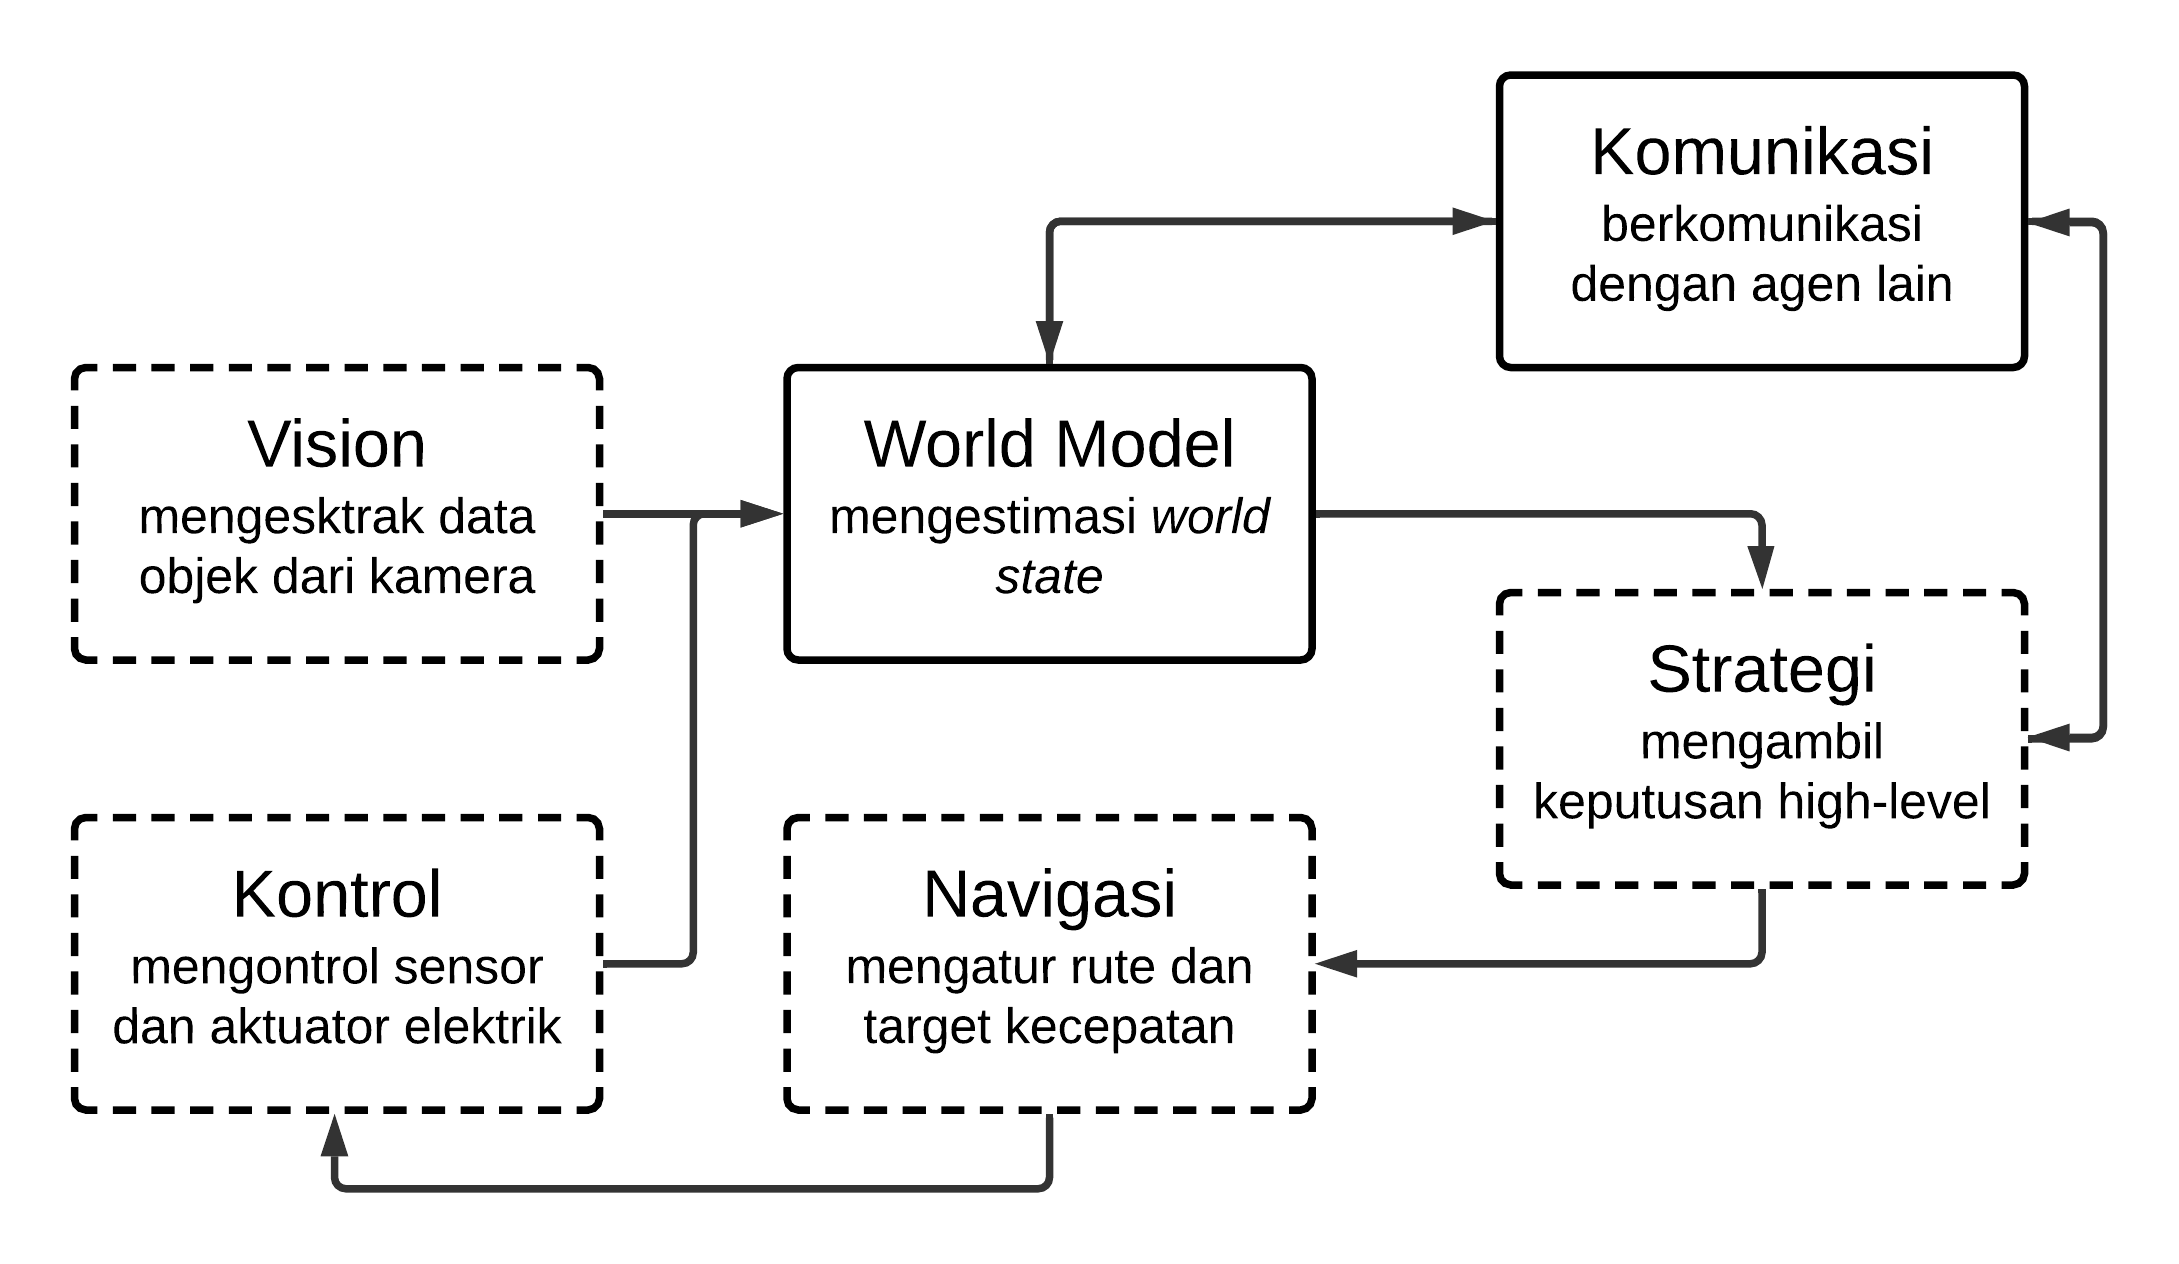
\includegraphics[width=0.8\textwidth]{resources/dagozilla-structure.png}
    \caption{Struktur modul Dagozilla}
    \label{fig:dagozilla-structure}
\end{figure}

Lingkungan perangkat lunak DAGOZILLA menggunakan \textit{platform} \textit{Robot Operating System} (\textit{ROS}) yang memungkinkan komunikasi antar proses oleh modul-modul aplikasi yang menjalankan fungsi-fungsi robot menggunakan paradigma \textit{publish-subscribe} pesan atau \textit{request-response} \textit{service} yang disediakan suatu modul. Modul-modul yang ada digambarkan pada gambar \ref{fig:dagozilla-structure}.

Fokus utama dari tugas akhir ini adalah mengembangkan modul \textit{world model} yang bertugas untuk memproses semua data persepsi dari modul sebelumnya maupun informasi dari robot lain untuk menyediakan estimasi keadaan dunia yang seakurat dan sefaktual mungkin agar dapat digunakan dalam melakukan pengambilan keputusan.

Modul kontrol berkomunikasi dengan mikrokontroler yang berhubungan langsung dengan \textit{hardware} untuk mengontrol aktuator dan mengambil data dari sensor-sensor lokal, diantaranya odometri motor penggerak dan kompas. Odometri mengukur perputaran yang dilakukan masing-masing roda penggerak yang dapat diolah menjadi data perpindahan dan kompas mengukur orientasi global dari robot itu sendiri.

Modul \textit{vision} mengekstrak data dari kamera, diantaranya posisi bola dari gambar menggunakan deteksi warna dan momen objek, dan sebaran titik dari garis lapangan maupun objek penghalang lapangan menggunakan algoritma \textit{radial search line}.

Semua data tersebut yaitu posisi bola, sebaran titik garis lapangan dan objek penghalang, data odometri dan kompas menjadi masukan untuk modul \textit{world model} lokal untuk mengestimasi \textit{world state} mencakup kinematika robot tim sendiri, posisi bola, dan robot musuh.

Posisi robot sendiri dikalkukasi menggunakan algoritma \textit{Augmented Monte Carlo localization} dengan masukan data perpindahan odometri untuk tahap prediksi dan data posisi garis lapangan dan kompas untuk tahap perbaruan pengukuran. Data yang lain seperti posisi bola dan posisi objek penghalang dipindahkan ke dalam \textit{frame global} menggunakan hasil lokalisasi tersebut sebagai masukan dari tahap sebelumnya.

\section{Analisis Solusi}

Salah satu pertimbangan dalam mengembangkan algoritma ini adalah bahwa masing-masing robot tetap harus selalu melakukan estimasi sendiri menggunakan data persepsi lokal robot tersebut. Hal ini dilakukan agar masing-masing robot harus tetap memiliki estimasi informasi krusial seperti posisi robot sendiri, bola, ataupun penghalang walaupun terjadi kegagalan jaringan komunikasi. Algoritma secara umum harus berjalan secara \textit{online} tanpa masing-masing robot harus menunggu informasi dari robot lain terlebih dahulu sebelum dapat dijalankan. Pemodelan informasi secara probabilistik terbukti dapat menjaga ketahanan akurasi estimasi dan memudahkan integrasi data baru menggunakan prinsip penapis Bayes. Data pengukuran yang didapat harus selalu diintegrasi dengan estimasi yang sudah ada.

Dalam pengiriman informasi, mengirimkan keseluruhan data pengukuran secara mentah ditinjau kurang dapat diandalkan dan meningkatkan beban komputasi untuk semua robot, melihat ada data seperti persepsi garis lapangan dan objek penghalang yang terdiri dari puluhan sampai ratusan data titik. Data seperti sebaran partikel estimasi seperti dalam algoritma penapis partikel haruslah diproses dahulu ke bentuk lain seperti \textit{Gaussian Mixture Model} sebelum disebarkan ke robot lain.

Data hasil pemrosesan harus mengandung \textit{time-stamp} agar robot yang menerima dapat mendeteksi dan melakukan pengolahan tambahan untuk data yang terlambat. Data juga mengandung ukuran tingkat kepercayaan keakuratan yang ditetapkan robot sumber karena walaupun pertukaran informasi dapat meningkatkan akurasi, hal tersebut juga dapat menyebabkan penyebaran \textit{error} dalam estimasi, sehingga harus didesain sehingga informasi dengan tingkat kepercayaan yang rendah tidak terlalu mempengaruhi informasi dengan tingkat kepercayaan yang lebih tinggi.

Dalam penanganan data yang di luar urutan karena keterlambatan, pendekatan melakukan penghitungan ulang dengan menyisipkan data terlambat tersebut dalam urutan sebenarnya ditinjau tidak terlalu efektif, karena mungkin mengakibatkan kebutuhan komputasi ulang banyak data, dan berdasarkan asumsi Markov, estimasi \textit{world state} dari penapis Bayes yang terbaru sudah mencakup semua informasi persepsi yang terintegrasi sebelumnya, sehingga fokus dari desain algoritma diarahkan ke bagaimana cara menggunakan data yang terlambat tersebut sehingga dapat diintegrasi ke estimasi yang sudah ada sekarang.

Penggunaan algoritma \textit{supervised learning} dapat diimplementasikan menggunakan luaran dari simulator tetapi pemilihan algoritma yang digunakan membutuhkan banyak pertimbangan, seperti waktu komputasi, jenis estimasi sekuensial yang terus-menerus dengan kemungkinan data di luar urutan, dan sifat beberapa algoritma yang bersifat \textit{black box} yang tidak bisa divalidasi kebenarannya membawa faktor risiko keamanan yang penting di bidang robotika.

\section{Rancangan Lingkungan Simulasi}

Dalam pembangunan model simulasi, digunakan beberapa instans dari modul \textit{world model} yang sama dengan yang akan diimplementasikan di lingkungan DAGOZILLA, dengan kebutuhan untuk mensimulasikan keadaan dunia sebenarnya, persepsi sensor dengan profil \textit{error} tertentu, modul komunikasi antar modul \textit{world model} dengan kemungkinan latensi, dan modul yang mengevaluasi kinerja dari algoritma dalam berbagai skenario.

Diagram arsitektur lingkungan simulasi digambarkan di \ref{fig:simulation-structure}. Simulasi mengandalkan modul-modul terpusat untuk mensimulasikan keadaan dunia dan sensor, komunikasi berlatensi, dan mengevaluasi kinerja algoritma. Modul dijalankan di \textit{ROS} dengan pemetaan ulang topik untuk membedakan pesan ke masing-masing instans modul \textit{world model}.

\begin{figure}[h]
    \centering
    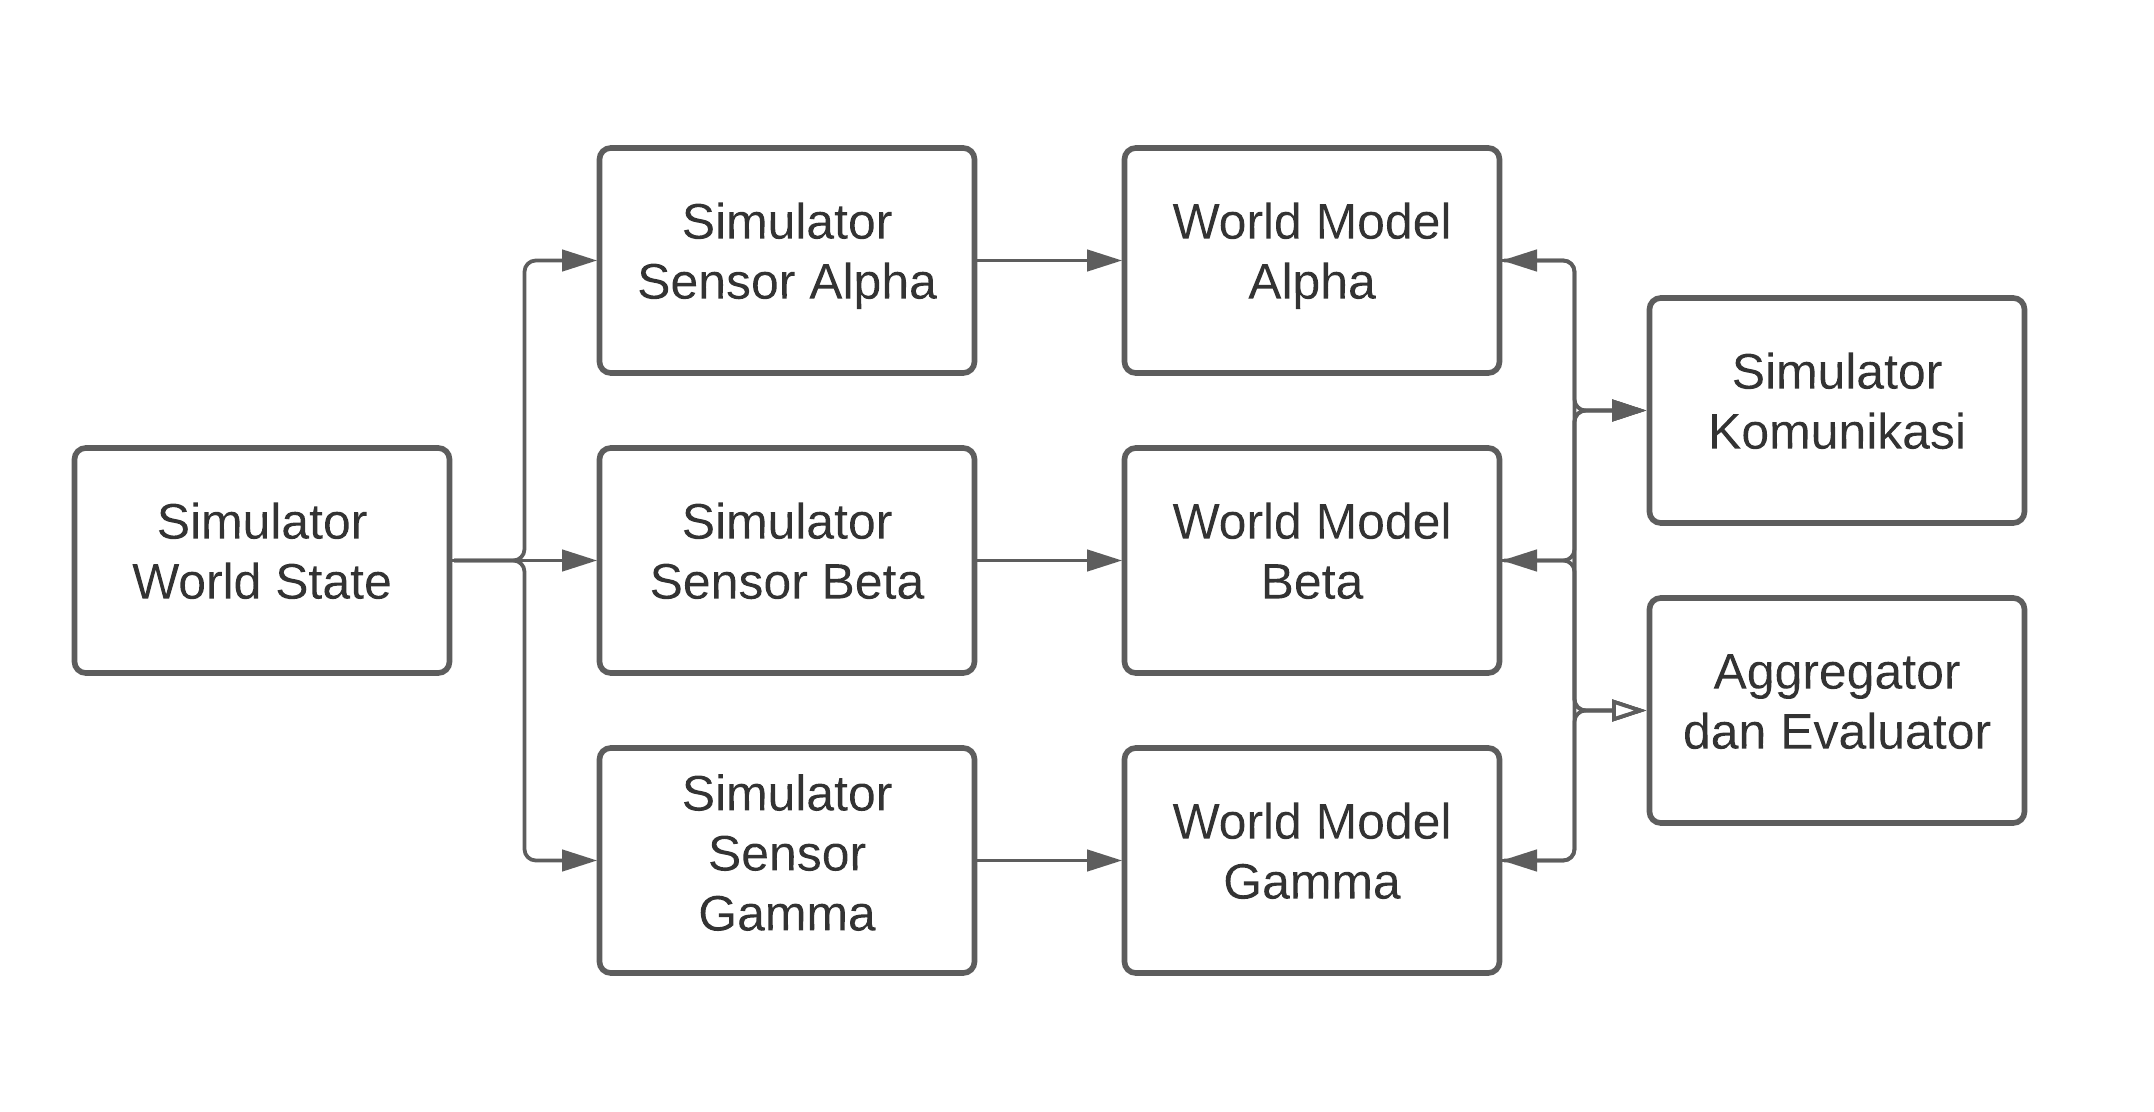
\includegraphics[width=0.8\textwidth]{resources/simulation-structure.png}
    \caption{Struktur modul simulasi}
    \label{fig:simulation-structure}
\end{figure}

Modul simulator \textit{world state} dan sensor menentukan konfigurasi posisi dan kinematika masing-masing robot dan bola berdasarkan skenario untuk diturunkan menjadi hasil persepsi masing-masing robot berdasarkan profil \textit{error} dari sensor tersebut. Modul simulator komunikasi dengan latensi menerima informasi \textit{world state} yang dikirim dari modul-modul \textit{world model} yang ada lalu menyimpan dan menyebarkannya ke modul \textit{world model} lainnya dengan latensi berdasarkan skenario. Modul evaluator lalu menerima membandingkan hasil estimasi setiap modul dengan nilai kebenaran dari simulator \textit{world state} untuk menghitung kinerja dari algoritma yang diimplementasi.

Skenario gerakan posisi dari robot dan bola memodelkan gerakan robot dan bola di pertandingan sebelumnya dengan formasi dua penyerang dan satu penjaga gawang dalam skenario seperti \textit{kick-off}, bola mati, tahap menyerang, dan bertahan. Skenario latensi komunikasi terdiri dari keadaan latensi rendah dalam keadaan normal, keadaan gangguan komunikasi dalam jaringan untuk semua robot, dan gangguan untuk suatu robot secara spesifik. Evaluasi algoritma dihitung dari akurasi posisi bola dan objek yang diestimasi dengan keadaan nyata yang didapat dari modul simulator \textit{world state}.

\section{Rancangan Solusi}

Diagram alir hipotesis solusi digambarkan di \ref{fig:solution-flowchart}, dimana estimasi dalam satu siklus dilakukan dengan pertama memproses data persepsi lokal, menyebarkan informasi ke jaringan, dan mengintegrasi informasi yang tersedia dari robot lain. Alternatif yang diimplementasi adalah penggunaan penapis kalman atau penapis partikel dalam memproses data lokal. Integrasi data yang terlambat dilakukan menggunakan modifikasi data yang terlambat tersebut untuk mengestimasi posisi kandidat dari objek di waktu sekarang.

Dalam menyesuaikan waktu untuk data yang terlambat, robot yang melakukan pengukuran data terkait juga mengestimasi kecepatan dari objek yang diukur menggunakan regresi linear beberapa data terakhir atau ikut diestimasinya kecepatan tersebut dalam keadaan objek yang ditapis dalam algoritma Kalman atau partikel yang digunakan. Penyesuaian waktu kemudian dilakukan menggunakan estimasi sederhana menggunakan informasi posisi dan kecepatan lampau yang ada dengan mengasumsikan kecepatan tersebut konstan.

\begin{figure}[h]
    \centering
    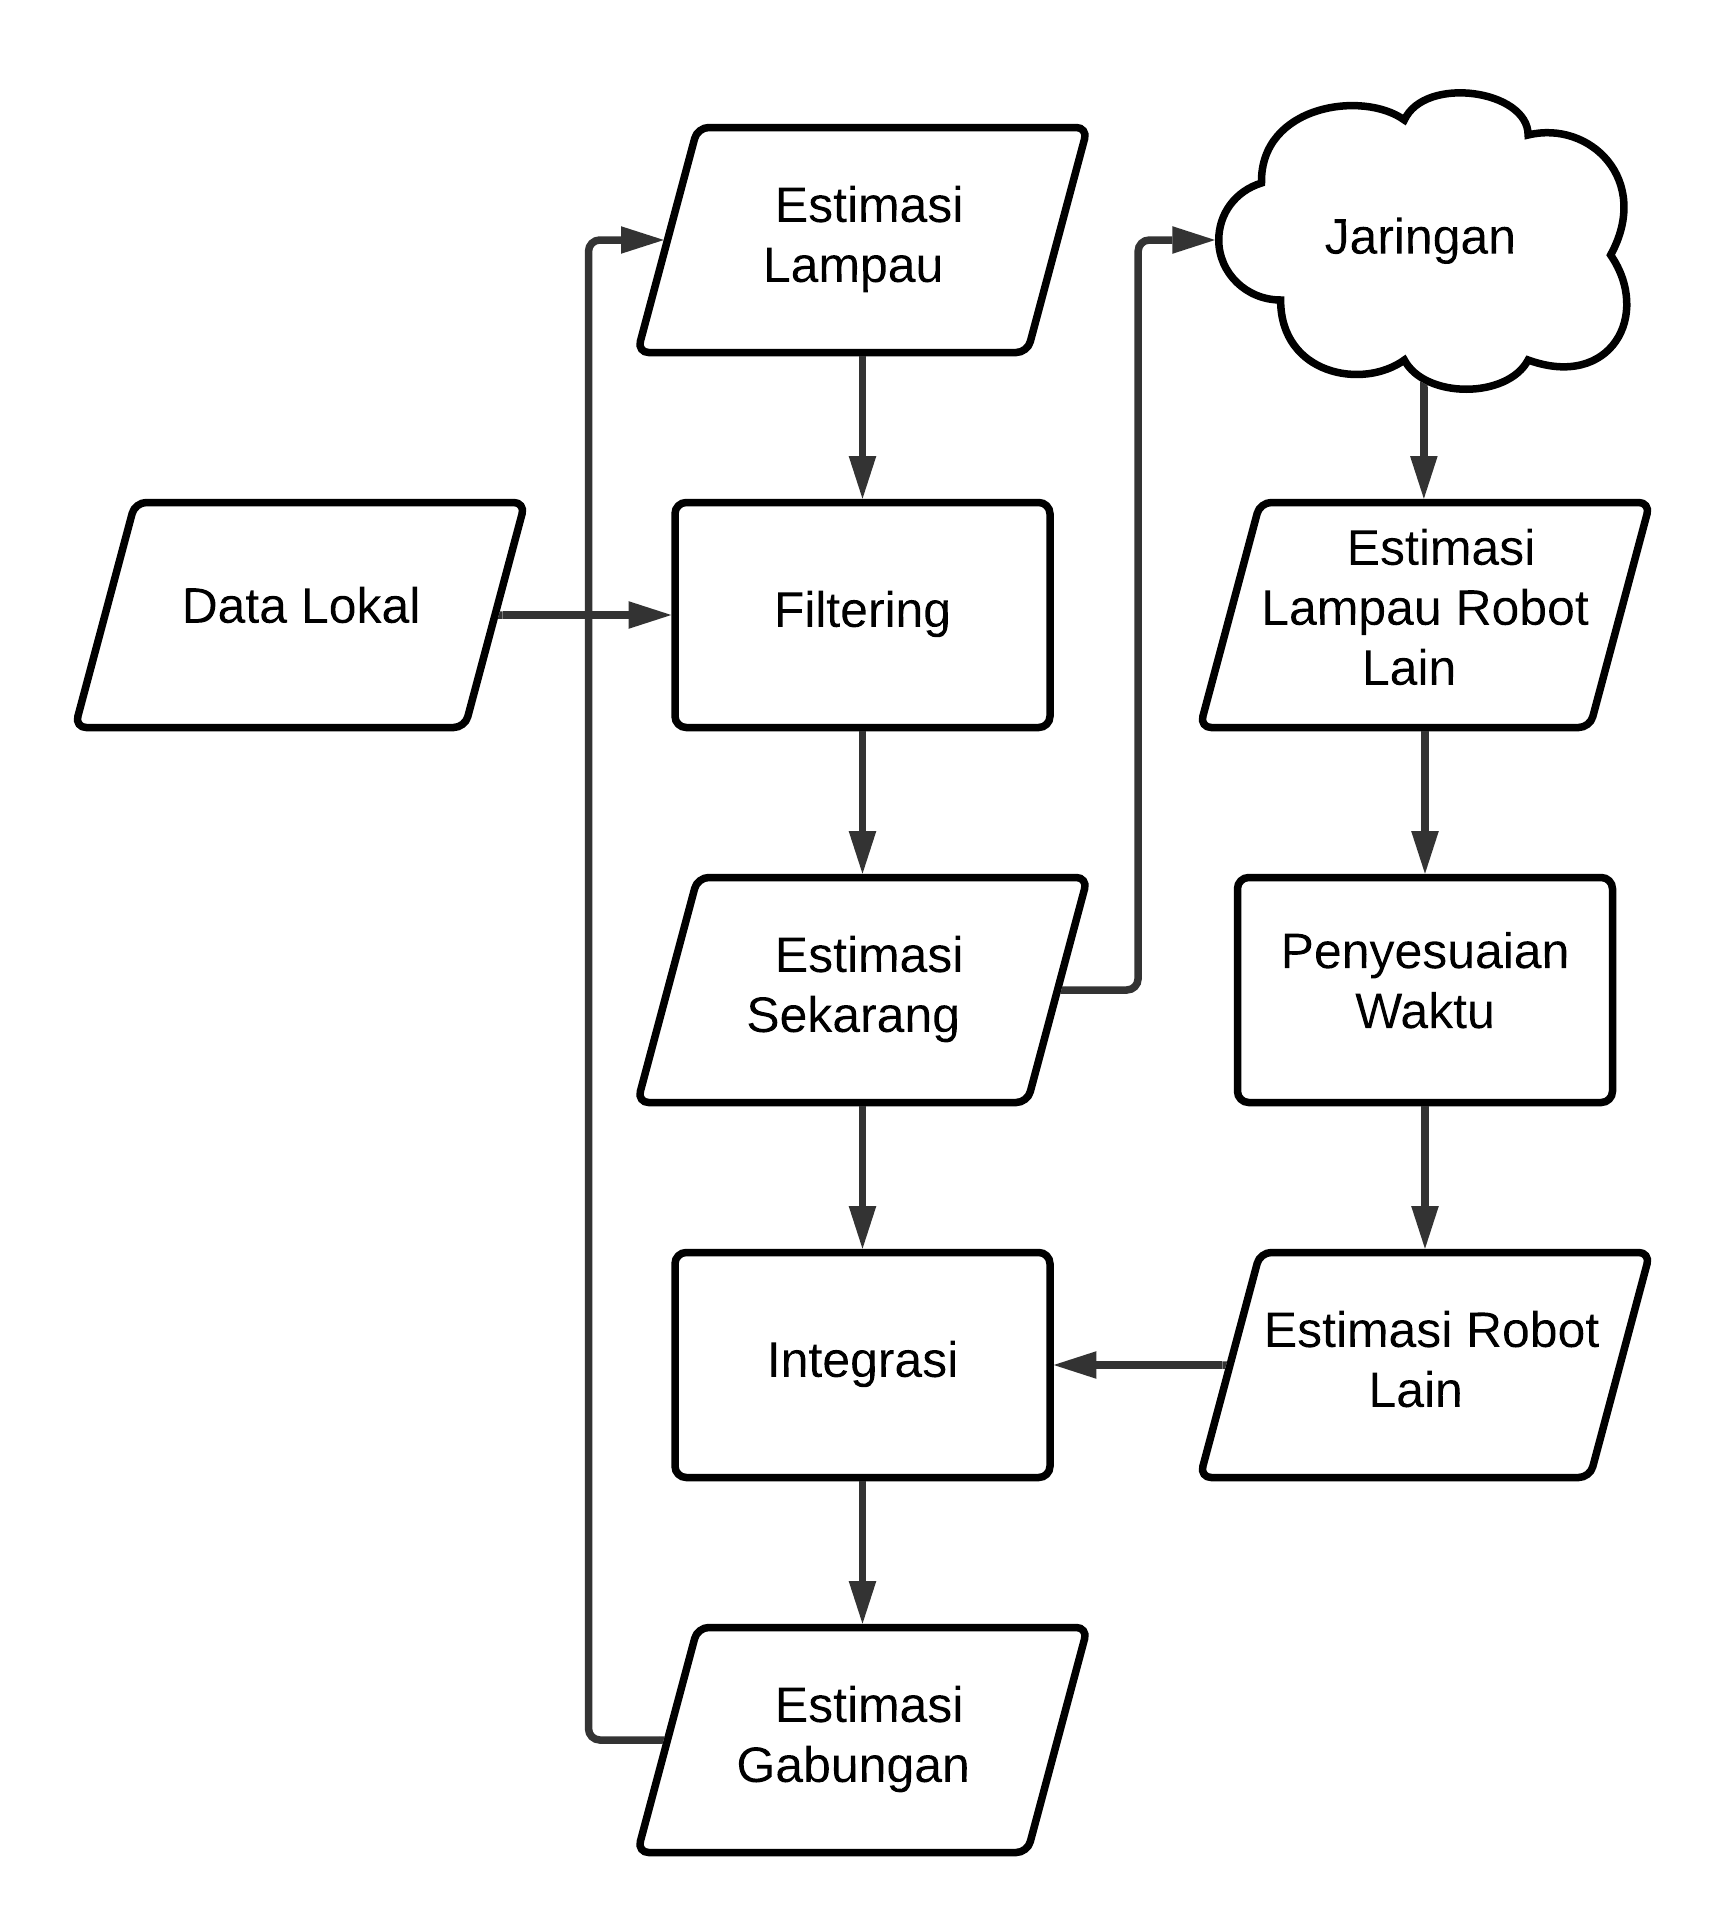
\includegraphics[width=0.8\textwidth]{resources/solution-flowchart.png}
    \caption{Diagram alir hipotesis solusi}
    \label{fig:solution-flowchart}
\end{figure}
